% -*- TeX-master: "all_the_notes.tex" -*-

\section{Quantum Electrodynamics Formalism\label{subsec:l2-CPB}}

   \subsection{Superconductors}
   In  superconductors CP  carry charge.   What happens  is that  the
   Fermi level  splits into  2 bands that  are $\pm\Delta$  above and
   below $E_F$, and  each electron in the CP belongs  to one of these
   bands.


   {{ Phase is quantised in a sc loop
       \begin{equation}
         \begin{aligned}
           \phi  = \phi_\text{ext}  + 2\pi  N  \Leftrightarrow \Phi  = \Phi_\text{ext}  +
           \Phi_0 \\(\Phi_0 = \frac{h}{2e}, \Phi/\Phi_0=\phi/2\pi)
         \end{aligned}
       \end{equation}
     }}

   \subsection{Josephson junction}
   Now work  with JJ.   The states  on the  two sides  of the  JJ are
   $\left|\psi_0\right|e^{i\phi_1}$                               and
   $\left|\psi_0\right|e^{i\phi_2}$.     Solving   the    Schrodinger
   equation for the condensate state, when E=0

   \begin{equation}
     -\frac{\hbar^2}{2m}\iderivative{^2}{x^2}\psi+U\psi = 0 \Rightarrow
     \left\lbrace\begin{aligned}
         \psi & = A_0e^{-kx}+B_0e^{+kx}\\
         k & = \frac{\sqrt{2mU}}{\hbar}
       \end{aligned} \right. \Rightarrow \left\lbrace\begin{aligned}
         \psi & = A\cosh(kx)+B\sinh(kx)\\
         k & = \frac{\sqrt{2mU}}{\hbar}
       \end{aligned} \right.
   \end{equation}

   \noindent           Apply            BC           for           JJ
   $\psi(a/2)       =       \left|\psi_0\right|e^{i\phi_2}$       and
   $\psi(-a/2) = \left|\psi_0\right|e^{i\phi_1}$ to find that

   \begin{align}
     A &= \frac{\left|\psi_0\right|}{\cosh(ka/2)}\\
     B &= \frac{\left|\psi_0\right|}{\sinh(ka/2)}.
   \end{align}

   \noindent {The super current is then}

   \begin{equation}
     I = -\frac{i\hbar}{2m}(2e)\left[\psi^*\iderivative{\psi}{t}-\psi\iderivative{\psi^*}{t}\right] \equiv -\frac{2e\hbar}{m}\text{Im}\left[\psi^*\iderivative{\psi}{t}\right],
   \end{equation}

   \noindent  at $x=0$  can  be  evaluated, as  can  the voltage  and
   energy, which results in a phase dependence

   \begin{equation}
     \label{eq:jj-current-and-voltage}
     I = I_c\sin(\phi_2-\phi_1); \qquad \frac{d\phi}{dt} = \frac{2e}{\hbar}V
   \end{equation}

   The phase across the  JJ in a circuit is the  phase induced by the
   external flux i.e.

   \begin{equation}
     \label{eqn:l2-phasesum}
     \phi_1+\phi_2+\ldots = \phi_\text{ext} = \frac{\Phi_\text{ext}}{\Phi_0}2\pi,
   \end{equation}

   \begin{equation}
     \left\lbrace\begin{aligned}
         I &= I_c\sin(\phi_2-\phi_1)\equiv I_c\sin(\phi)\\
         V&=\dot{\Phi} \equiv \frac{\dot{\phi}}{2\pi}\Phi_0
       \end{aligned}\right.  \Rightarrow U =
     \left\lbrace\begin{aligned}
         \int_{0}^{t}IV dt & = \int_{0}^{t}I_c\sin(\phi)\frac{\Phi_0}{2\pi}\frac{d\phi}{dt}dt\\
         & = \int_{0}^{\phi} E_J\sin(\phi)d\phi\\
         &       \red{=       E_J(1-\cos(\phi)),\qquad       E_J       =
           \frac{\Phi_0I_c}{2\pi}.}
       \end{aligned}\right.
     \label{l2-JJEnergy}
   \end{equation}

  \begin{center}
    Increase  $  I $  \ira  Increase  $  \phi  = \phi_2-\phi_1  $  to
    $ \pi/2 $  \ira Increse energy $ U $  \ira \textbf{at some point,
      we reach  critical currrent  and highest  energy -  beyond this
      limit, we will generate voltage}


\begin{figure}[h]
  \centering 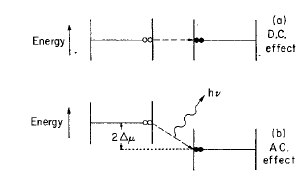
\includegraphics[height=3cm]{josephson_effecti}
\end{figure}

\noindent
\end{center}

\paragraph{Inductance} is found by performing:

\begin{itemize}
\item Suppose  a change in current,  $ \delta_I $ causes  a change in
  phase $ \delta_1\phi $:

    \begin{equation}
      I_0 + \delta_I = I_c\sin(\phi_0+\delta_\phi) \iRa \delta_I = \purple{I_c\cos(\phi_0)\delta_\phi.}
    \end{equation}
  \item The voltage across the junction:
    \begin{equation}
      V = \frac{\dot{\phi}}{2\pi}\Phi_0 = \frac{\Phi_0}{2\pi}\left(\red{\dot{\phi}_0} + \dot{\delta}_\phi\right) =  \frac{\Phi_0}{2\pi}\purple{\frac{\dot{\delta}_I}{I_c\cos(\phi_0)}}.
    \end{equation}

  \item FInally expressing the inductance

    \begin{equation}
      L = V/\frac{dI}{dt} = V/\dot{\delta}_I = \frac{\Phi_0}{2\pi}\frac{1}{I_c\cos(\phi_0)}.
    \end{equation}
  \end{itemize}

  \begin{framed}\noindent
    \begin{equation}\label{eq:jj-inductance}
      L_J = \Phi/I =
      \frac{\Phi_0}{2\pi}\frac{1}{I_c}\frac{1}{\cos(\phi_0)}
    \end{equation}
  \end{framed}

  \noindent The current is given by:

   \begin{equation}\label{introducing-qed-operators-critical-current}
     I_cR_n = \frac{\pi\Delta(T)}{2e}\tanh\big(\frac{\Delta(T)}{2k_bT}\big),
   \end{equation}

   \noindent derived from BCS theory for a superconducting energy gap
   of $ \Delta(T) $ and normal resistance $ R_n $ of the JJ.

   \paragraph{Critical current $ I_c $}
   Taking the limit of $ T\ira0 $ we get

   \begin{equation}\label{app:criticalCurrent}
     I_cR_n = \frac{\pi\Delta(0)}{2e}
   \end{equation}


   \begin{framed}\noindent
     \paragraph{Josephson  Energy  from  JJ  parameters}  Subbing  in
     Eq.~\eqref{app:criticalCurrent} into Eq.~\eqref{l2-JJEnergy}:

     \begin{equation}
       \begin{aligned}
         E_J & = \frac{R_q}{R_n}\frac{\Delta(0)}{2}\\
         R_n & = 1.84\,\text{k}\Omega \text{ for 100 } \times 100\,\text{nm}^2\\
       \end{aligned}
     \end{equation}

     \noindent with  $ R_q =  \frac{h}{(2e)^2} $. The larger  the JJ,
     the lower  the resistance of  the junction and hence  the bigger
     the Josephson energy.

     \red{JJ resistance increases  by $ \sim 10\% $ as  one goes from
       room to cryogenic temperatures.}
   \end{framed}

   \subsubsection{Inductance energy}
   Inductance             energy             derives             from
   $                       \frac{\Phi_L^2}{2L}                      =
   \frac{\Phi_0^2}{(2\pi)^22L}(\phi_\text{ext}-\phi_J)^2            =
   E_L(\phi_\text{ext}-\phi_J)^2 $

   \begin{equation}
     \begin{aligned}
       E_L & = \frac{\Phi_0^2}{(2\pi)^22L}\\
       L     &      \propto     R_n     =      \iunit{1.5}{nH     per
         100}\times\iunit{100}{nm}^2
     \end{aligned}
   \end{equation}

   \subsubsection{Summary of energies}
   \begin{table}[h]
     \centering {%
       \footnotesize%
       \begin{tabular}{|c|c|p{6cm}|c|}%
         \hline\textbf{Energy}    &    &    \textbf{Variable   parameter}    &    \textbf{Energy
                                                                               ($  N_{sq}=10,  N_{NbN} =  5$)}
         \\\hline
         $ E_J $ & $ \frac{R_q}{R_n}\frac{\Delta(0)}{2} $ & $ R_q = \frac{h}{(2e)^2} = 6.484\,\text{k}\Omega,\newline \Delta = 1.73*(k_b\times 1.3\,\text{K}) = 3.1\times10^{-23}, \newline R_n = \iunit{18.4}{k}\Omega \text{ for $100 \times 100\,\text{nm}^2$}  $ & \iunit{77.5}{GHz} \\
         $ E_C $ & $ \frac{(2e)^2}{2CN_{sq}} $ & $ \varepsilon = 10, d = \iunit{2}{nm}, \newline A = 100\times\iunit{100}{nm}^2, \newline C = \frac{\varepsilon\varepsilon_0A}{d} = \iunit{0.5}{fF} $ & \iunit{17.4}{GHz} \\
         $      E_L       $      &      $      \frac{\Phi_0^2}{(2\pi)^22LN_{NbN}}       $      &
                                                                                                 $\Phi_0
                                                                                                 =2\times{-15}\,\text{Wb},\newline
                                                                                                 L
                                                                                                 =
                                                                                                 \iunit{1.5}{nH}
                                                                                                 $
                                                                                                 per
                                                                                                 NbN
                                                                                                 square
                                                                             &
                                                                               \iunit{16.2}{GHz}\\\hline
       \end{tabular}
     }
   \end{table}

   \subsection{JJ Brief summary}
   \label{sec:jj-brief-summary}

\begin{framed}\noindent
  Up      to     this      point     we      have     found      from
  (\autoref{eq:jj-current-and-voltage})
  \begin{equation}
    I = I_c\sin(\phi_2-\phi_1); \qquad \frac{d\phi}{dt} = \frac{2e}{\hbar}V
  \end{equation}

  \noindent So a constant voltage will result in an AC current across
  the JJ. The JJ itself will be modelled by
  \begin{equation}\label{eq:jj-total-current}
    \begin{aligned}
      I(t) & = \red{\text{JJ current}} + \green{\frac{d}{dt}\left[ CV \right]} + \blue{\frac{V}{R}}\\
      & = \red{I_c\sin\varphi} + \frac{\Phi_{0}}{2\pi}\left[ \green{C
          \frac{d^2\varphi}{dt^{2}}}                                +
        \blue{\frac{1}{R}\frac{d\varphi}{dt}} \right]
    \end{aligned}
  \end{equation}

  \noindent as shown in \autoref{fig:typical_jj_setup}.
\end{framed}

\subsection{Shapiro steps}
\label{sec:shapiro-steps}

\textbf{Now, let  us irradiate the  JJ with a frequency  $f_1$:} This
will drive a voltage

\begin{equation}
  \begin{aligned}
    V & = V_0 + V_1\cos\left(2\pi f_1 t  \right)\\
  \end{aligned}
\end{equation}

\noindent driving a phase change

\begin{equation}
  \begin{aligned}
    \iabs{\frac{d\delta}{dt}} & = \frac{2eV_0}{\hbar} +
    \frac{2eV_{1}}{\hbar}\cos\left(  2\pi f_1  t \right)  \\
    \Rightarrow \phi &  = \red{\phi_0} + \green{\frac{2eV_0}{\hbar}t}
    + \blue{\frac{2eV_{1}}{\hbar}\frac{1}{2\pi
        f_{1}}\sin\left( 2\pi f_1 t \right)} \\
    & = \red{\phi_0} + \green{\frac{2eV_0}{\hbar}t} +
    \blue{\alpha\sin\left( 2\pi f_1 t \right)} \\
  \end{aligned}
\end{equation}

\noindent  where   due  to  the   high  frequency  and   finite  $V$,
\blue{$\alpha  = \frac{2eV_{1}}{2\pi  f_1} <<  1$ }.   This drives  a
current

\begin{equation}
  \begin{aligned}
    I & = I_0\sin\left(\red{\phi_0} + \green{\frac{2eV_0}{\hbar}t} +
      \blue{\alpha\sin\left( 2\pi f_1 t \right)} \right) \\
    &     \approx     I_0     \left[     \sin\left(\red{\phi_0}     +
        \green{\frac{2eV_0}{\hbar}t}\right)  + \blue{\alpha\sin\left(
          2\pi    f_1    t    \right)}\cos    \left(\red{\phi_0}    +
        \green{\frac{2eV_0}{\hbar}t} \right) \right].
  \end{aligned}
\end{equation}

\noindent Term by term:

\begin{itemize}
\item $\sin\left(\red{\phi_0}  + \green{\frac{2eV_0}{\hbar}t}\right)$
  averages to 0.
\item
  $\blue{\sin\left(  2\pi  f_1  t \right)}\cos  \left(\red{\phi_0}  +
    \green{\frac{2eV_0}{\hbar}t} \right)$  will only  be non  zero if
  the    arguments    of    $\sin$     and    $\cos$    are    equal:
  $\int_0^T\sin(\beta          t)\cos(\beta           t)dt          =
  \frac{1}{2}\int_0^{T}\sin(2\beta   t)dt  =   \frac{1}{4\beta}\left[
    \cos(2\beta  t) \right]_T^0  \ne  0 $  which  apparently gives  a
  non-zero average.

  \begin{framed}\noindent
    Therefore there is a set of frequencies
    \begin{equation}
      2\pi f_{1} = \frac{2eV_{0}}{\hbar}n, n \in \mathbb{Z}
    \end{equation}
    at which the current
    \begin{equation}
      I = \text{Some constant} \times \alpha \times I_0, \quad \alpha = \frac{2eV_{1}}{2\pi  f_1}
    \end{equation}

    \noindent takes on a finite value. These are the Shapiro steps.
  \end{framed}
\end{itemize}

\begin{figure}[h]
  \centering \inkfig{8cm}{jj_shapiro_step_at_frequency}
  \caption{\small Shapiro steps 0 there is a non zero current at some
    frequencies       for       a      given       bias       voltage
    $V_0$. \label{fig:jj_shapiro_step_at_frequency}}
\end{figure}


\subsection{Effective "ball" system}
\label{sec:effect-ball-syst}

Now if we rewrite ~\autoref{eq:jj-total-current}

\begin{equation}\label{eq:jj-force-equation}
  I = \red{I_c\sin\varphi} + \frac{\Phi_0}{2\pi}\left[ \green{C
      \frac{d^2\varphi}{dt^{2}}}                                +
    \blue{\frac{1}{R}\frac{d\varphi}{dt}} \right]
\end{equation}

\noindent in another form where  we defined a characteristic time for
the system

\begin{equation}
  \tau = \frac{2\pi}{\Phi_0}I_cR t  \qquad \Rightarrow \qquad \frac{d\tau}{dt} = \frac{2\pi}{\Phi_0}I_cR.
\end{equation}

\noindent resulting in

\begin{equation}\label{eq:jj-damping}
  \begin{aligned}
    \frac{I}{I_c} &= \red{\sin\delta} + \green{\beta_{c} \frac{d^2\delta}{d\tau^2}} + \blue{\frac{d\delta}{d\tau}} \\
    & \left\lbrace
      \begin{aligned}
        \beta_c & = \frac{2\pi}{\Phi_0}I_cR^2C\\
        \frac{I_c}{\Phi_0} & = \textbf{has units of inductance}
      \end{aligned}
    \right.    \Rightarrow  \beta_c   =  \frac{R^2C}{L_J}   =  \left(
      \omega_pRC  \right)^2 =  Q^2  \qquad \text{where  } \omega_p  =
    \frac{1}{\sqrt{L_JC}} \text{=plasma frequency}
  \end{aligned}
\end{equation}

\noindent where $\beta_c$ is associated with the quality factor.
\begin{itemize}
\item  $\beta_c>> 1$  (underdamped), phase  is very  mobile and  thus
  suffers from hysteresis
\item $\beta_c << 1$ (overdamped), large energy dissipation.
\end{itemize}

This can  be envisaged as a  ball on a tilted  washboard potential by
integrating the effective force equation over $\delta$

\begin{equation}
  \underbrace{I - I_c\sin(\delta)}_{\text{non-linear restoring force}} = \underbrace{ \frac{\Phi_{0}}{2\pi}C}_{\text{mass}}\underbrace{\frac{d^2\delta}{dt^2}}_{\text{acceleration}} + \underbrace{\frac{\Phi_{0}}{2\pi}\frac{1}{R}\frac{d\delta}{dt}}_{\text{drag force}}
\end{equation}

\noindent to get the potential landscape:

\begin{equation}
  U(\delta) = I\delta - I_c\cos(\delta).
\end{equation}

\noindent The potential is a washboard with 2 cases
\begin{itemize}
\item $I=0$ and no current flows
\item $I>I_c$  and there the  ``$\delta$'' particle is free  to move,
  meaning  that $\frac{d\delta}{dt}  \ne  0$ and  there  is a  finite
  voltage  across  the  junction.   \textbf{This is  the  JJ  current
    exceeding  the critical  value  and the  JJ  turning into  normal
    state}.
\end{itemize}

\begin{figure}[h]
  \centering \inkfig{8cm}{jj_washboard}
  \caption{\small      Phase      exists     on      a      washboard
    potential\label{fig:jj_washboard}}
\end{figure}

\subsection{SQUID to control $ E_J $\cite{zhu2010}}
\begin{framed}\noindent
  Inductance of a SQUID:
  \begin{equation}\label{l2:squid:inductance}
    L_J(\Phi_\text{ext}) = V/\frac{dI}{dt} = \frac{\hbar}{4eI_c|\cos(\pi\Phi_\text{ext}/\Phi_0)}.
  \end{equation}
\end{framed}

Two JJ in a loop give a total current

    \begin{equation}
      I = I_{c1}\sin(\phi_1)+I_{c2}\sin(\phi_2),
    \end{equation}

    \noindent  which  along  with the  phase  quantisation  condition
    Eq.\eqref{eqn:l2-phasesum} and  symmetric JJs $I_{c1}=I_{c2}=I_c$
    results in

    \begin{equation}
      \begin{aligned}
        I = & I_{cs}(\Phi_\text{ext})\sin(\phi)\\
        & I_{cs} = 2I_c|\cos(\pi\Phi_\text{ext}/\Phi_0)|\\
        & \phi = (\phi_1+\phi_2)/2
      \end{aligned},
    \end{equation}

    \noindent      which     has      a      similar     form      to
    Eq.\eqref{eq:jj-current-and-voltage},   but   now  the   critical
    current $I_{cs}$ is  controlled by an external  field. Taking the
    derivative

    \begin{equation}
      \begin{aligned}
        \frac{dI}{dt}=2I_{cs}(\Phi_\text{ext})\cos(\phi)\frac{d\phi}{dt},
      \end{aligned}
    \end{equation}

    \noindent      and     expressing      the     voltage      using
    Eq.\eqref{eq:jj-current-and-voltage}         and         assuming
    $\cos(\phi)\approx1$ for small excitations

    \begin{equation}
      V = \frac{\hbar}{2e}/\frac{d\phi}{dt} = \frac{\hbar}{4eI_{cs}}\frac{dI}{dt},
    \end{equation}

    \noindent    from     which    one    finds     the    inductance
    ($\Phi     =     LI     \rightarrow      L     =     \frac{d\Phi}{dI}     =
    \frac{d\Phi}{dt}/\frac{dI}{dt}   =    V/\frac{dI}{dt}$for   small
    excitations

    \begin{equation}
      L_J(\Phi_\text{ext}) = V/\frac{dI}{dt} = \frac{\hbar}{4eI_c|\cos(\pi\Phi_\text{ext}/\Phi_0)}.
    \end{equation}
    \vspace{6ex}

    \begin{framed}\noindent
      Energy of two JJ forming a SQUID:
      \begin{equation}
        E_{J} = \sqrt{E_{J1}^2 + E_{J2}^2 + 2E_{J1}E_{J2}\cos\left( \frac{2e\Phi}{\hbar} \right)}
      \end{equation}

      \noindent and a chain of SQUIDs has inductance

      \begin{equation}
        L = \frac{N\hbar^{2}}{4e^2E_J}
      \end{equation}

      \noindent \textbf{\red{Only valid for  small currents not close
          to the critical current!}}
    \end{framed}

   \subsection{Building blocks for quantum circuits.}
   Quantum circuits are built from
   \begin{itemize}
   \item   JJs,    who   posses    an   inductance    $L_J$   defined
     Eq.\eqref{l2:squid:inductance}.  The energy  comes from the flux
     stored by the inductor
     \begin{equation}
       E_J(\Phi_\text{ext}) = \frac{\Phi_0}{2L_J(\Phi_\text{ext})}
     \end{equation}
   \item  An inductor  $L$ with  energy from  a the  flux inside  the
     inductor (coil)
     \begin{equation}
       E_L = \frac{\Phi^2}{2L}
     \end{equation}
   \item A capacitor with energy
     \begin{equation}
       E_c = \frac{Q^2}{2C}
     \end{equation}
   \end{itemize}

   \subsubsection{Kinetic Inductance}
   \label{sec:kinetic-inductance}

   \begin{framed}\noindent
     \red{\textbf{This   is   the   only  inductance   relevant   for
         superconductors!}}

     Drude  model is  the relationship  between current  and electric
     field due to  the finite relaxation time  (collision time, which
     is large in superconductors) of charge carriers $\tau$, it takes
     some time for a change in voltage to accelerate the particle.
     \begin{equation}
       \left\lbrace
         \begin{aligned}
           m \left\langle v \right\rangle & = qE\tau \\
           j & = nq \left\langle v \right\rangle
         \end{aligned}
       \right.
       \Rightarrow  j = \left(  \frac{nq^2\tau}{m} \right)E
     \end{equation}

     Complex conductivity
     \begin{equation}
       \sigma(\omega) = \frac{ne^2\tau}{m(1 - i\omega\tau)} = \frac{ne^2\tau}{m(1+\omega^2\tau^2)} - i\frac{ne^2\tau^2}{m(1+\omega^2\tau^2)}
     \end{equation}

     \noindent We  equate the kinetic  energy of cooper pairs  to the
     equivalent                    inductive                   energy
     ($(mv^{2})(n_slA)  = \frac{1}{2}L_KI^2$),  where  $l,A$ are  the
     dimensions of the wire and  $n_s$ the cooper pair concentration,
     so that
     \begin{equation}
       L_K = \frac{ml}{2n_se^2A}.
     \end{equation}

     \noindent     Transforming     conductivity     to     impedance
     $Z = \frac{L}{A}\frac{1}{\sigma}$:
     \begin{equation}
       Z = R + j\omega L_k.
     \end{equation}
   \end{framed}

   For the most general discussion, we compare

   \setlength{\extrarowheight}{4mm}
   \begin{table}[h]
     \caption{}
     \label{tab:conversion1}
     \begin{center}
       \begin{tabular}{|c|c|c|c|}
         \hline
         &\textbf{$ Q $ and $ \Phi $} & \textbf{Mechanical} & \textbf{$ V $ and $ I $} \\\hline
         \multicolumn{4}{|c|}{$ I =\dot{Q }\qquad V=\dot{\Phi} $}\\
         \multicolumn{4}{|c|}{$ Q=CV\qquad \Phi = LI $}\\\hline
         \multirow{2}{*}{Kinetic} & $ \frac{Q^2}{2C} $  & $ \frac{p^2}{2m} $ & \textit{\scriptsize Inductor}\\
         & \textit{\scriptsize Capacitor} & $ \frac{m\dot{x}^2}{2} $& $ \frac{LI^2}{2} = \frac{LC^2\dot{V}^2}{2}$ \\\hline
         Potential & $ \frac{\Phi^2}{2L} $ & $ \frac{kx^2}{2} $ & $\frac{CV^2}{2}$ \\
         & \textit{\scriptsize Inductor} & & \textit{\scriptsize Capacitor} \\\hline
         $ \omega_0 $ & $  \frac{1}{\sqrt{LC}} $ &$  \sqrt{\frac{k}{m}} $ &$  \frac{1}{\sqrt{LC}} $\\\hline
         \multirow{2}{*}{Energy} & $\frac{Q^2}{2C}+\frac{1}{2}C\omega_0^2\Phi^2$ & $\frac{p_m^2}{2m}+\frac{1}{2}m\omega_m^2x^2$ & \\
         & & $\frac{m}{2}\left(\dot{x}^2+\omega_0^2x^2\right)$  & $ \frac{LC^2}{2}\left(\dot{V}^2+\omega_0V^2 \right)$\\\hline
         Momentum & $ Q $ & $ p $ & $I =  C\dot{V} $\\\hline
         Coordinate & $ \Phi $ & x & V\\\hline
         Mass & $ C $ & $ m $ & $ LC^2 $\\\hline
         Stiffness & $ \frac{1}{L} $ & $ k $ & C\\\hline
         Solution &$ \Phi=Ae^{i\omega_0t}+Be^{-i\omega_0t} $ & $ x=Ae^{i\omega_0t}+Be^{-i\omega_0t} $ & $ V=Ae^{i\omega_0t}+Be^{-i\omega_0t} $\\\hline
       \end{tabular}
     \end{center}
   \end{table}

   \setlength{\extrarowheight}{4mm}
   \begin{table}[h]
     \caption{}
     \label{tab:conversion2}
     \begin{center}
       \begin{tabular}{|c|c|c|c|}
         \hline
         &\textbf{$ Q $ and $ \Phi $} & \textbf{Mechanical} & \textbf{$ V $ and $ I $} \\\hline
         Momentum & $ Q $ & $ p $ & $I =  C\dot{V} $\\\hline
         Coordinate & $ \Phi $ & x & V\\\hline
         Mass & $ C $ & $ m $ & $ LC^2 $\\\hline
         Stiffness & $ \frac{1}{L} $ & $ k $ & C\\\hline
         \multirow{2}{*}{Energy} & $\frac{Q^2}{2C}+\frac{1}{2}C\omega_0^2\Phi^2$ & $\frac{p_m^2}{2m}+\frac{1}{2}m\omega_m^2x^2$ & \\
         & & $\frac{m}{2}\left(\dot{x}^2+\omega_0^2x^2\right)$  & $ \frac{LC^2}{2}\left(\dot{V}^2+\omega_0V^2 \right)$\\\hline
         \multirow{3}{*}{$ \mathcal{H} $} & \multirow{2}{*}{$ \frac{\hbar\omega_0}{2}\left(\frac{Q^2}{Q_0^2}+\frac{\Phi^2}{\Phi_0^2}\right) $} &  \multirow{2}{*}{$ \frac{\hbar\omega_0}{2}\left(\frac{\hat{p}^2}{p_0^2}+\frac{\hat{x}^2}{x_0^2}\right) $} & \multirow{2}{*}{$ \frac{\hbar\omega_0}{2}\left(\frac{\hat{I}^2}{I_0^2}+\frac{\hat{V}^2}{V_0^2}\right) $}\\
         & & & \\
         & $ \Phi_0=\sqrt{\frac{\hbar\omega_0}{C}},\  Q_0 = \sqrt{\frac{\hbar}{C\omega_0}} $& $ x_0 = \sqrt{\frac{\hbar}{m\omega_0}},\ p_0 = \frac{\hbar}{x_0} $ & $ V_0 = \sqrt{\frac{\hbar\omega_0}{C}},\ I_0 = \sqrt{\frac{\hbar\omega_0}{L}} $ \\\hline
         & \parbox[c]{5cm}{$ \left[\hat{\Phi},\hat{Q}\right] = i\hbar $ since $ \Phi $ and $ Q $ are exactly $ x $ and $ p $}& $ \left[\hat{x},\hat{p}\right] = i\hbar $ & \parbox{5cm}{$ \left[\hat{\Phi},\hat{Q}\right] = \left[CV,LI\right]=i\hbar $ so $ \left[\hat{V},\hat{I}\right] = \frac{i\hbar}{LC}$}\\\hline
         & $ \hat{\Phi} $& $ \hat{x} $ & $ \hat{V} $\\\hline
         & $ \hat{Q}=-i\hbar\frac{d}{d\Phi} $& $ \hat{p} = -i\hbar\frac{d}{dx} $ & $ \hat{I} = -i\frac{\hbar}{LC}\frac{d}{dV} $\\\hline
         & \multirow{2}{*}{$ a^{\dagger} = \sqrt{\frac{C\omega_0}{2\hbar}}\left(\hat{\Phi}-i\frac{\hat{Q}}{C\omega_0}\right) $} & \multirow{2}{*}{$ a^{\dagger} = {\frac{1}{\sqrt{2}}}\left(\frac{\hat{x}}{x_0}-i\frac{\hat{p}}{p_0}\right) $} & \multirow{2}{*}{$ a^{\dagger} = {\frac{1}{\sqrt{2}}}\left(\frac{\hat{V}}{V_0}-i\frac{\hat{I}}{I_0}\right) $}\\
         & & & \\\hline
       \end{tabular}
     \end{center}
   \end{table}

   We  see that  in  either  case, we  are  working  with a  harmonic
   oscillator  system,   with  corresponding  raising   and  lowering
   operators.

   {\scriptsize As a reminder, an equation with the form
     \[
       \mathcal{H}                                                  =
       \frac{\hbar\omega_0}{2}\left(y^2-\frac{^2}{y^2}\right)
     \]

     \noindent can be rewritten as

    \[
      \mathcal{H}                                                   =
      \hbar\omega_0\left(a^{\dagger}a+\frac{1}{2}\right)=
      \hbar\omega_0\left(\hat{N}+\frac{1}{2}\right)
    \]

    with eigenstates and eigenenenergies

    \[
      \ket{\Psi}_n=\ket{n}                 \qquad                E_n=
      \hbar\omega_0\left(n+\frac{1}{2}\right).
    \]

    \noindent The raising and lowering operators act in the following
    way on the eigenstates

    \[
      \left\lbrace\begin{aligned}
          a\ket{n} & = \sqrt{n}\ket{n-1}\\
          a^{\dagger}\ket{n} &= \sqrt{n+1}\ket{n+1}\\
        \end{aligned}\right. \Rightarrow
      \hat{N}\ket{n}     =     a^{\dagger}    \sqrt{n}\ket{n-1}     =
      \sqrt{n}^2\ket{n}=n\ket{n} ,
    \]
    \noindent and  the matrix form,  evaluated by finding  the matrix
    coefficients $ c_{ij}=\bra{i}\hat{C}\ket{j} $

    \[
      \hat{a}=\begin{pmatrix}
        0 & \sqrt{1} & 0 & 0\\
        0 & 0 & \sqrt{2} & 0\\
        0 & 0 & 0 & \sqrt{3}\\
        0 & 0 & 0 & \ddots\\
      \end{pmatrix} \qquad a^{\dagger}=\begin{pmatrix}
        0 & 0 & 0 & 0\\
        \sqrt{0+1} & 0 & 0 & 0\\
        0 & \sqrt{1+1} & 0 & 0\\
        0 & 0 & \sqrt{2+1} & \ddots\\
      \end{pmatrix} \qquad \hat{N} =\begin{pmatrix}
        0 & 0 & 0 & 0\\
        0 & 1 & 0 & 0\\
        0 & 0 & 2 & 0\\
        0 & 0 & 0 & \ddots\\
      \end{pmatrix}
    \]
  }

  For the Harmonic oscillator which the system replicates, the energy
  levels  are   evenly  spaced,  making  it   impossible  to  address
  individual states.  But by replacing the inductor with a JJ

   \begin{equation}
     E_L = \frac{\Phi^2}{2L} \longrightarrow U = -E_J\cos(\phi),
   \end{equation}

   \noindent changing the quadratic to a cosine potential.
   \newpage
